\documentclass[hide notes,intlimits]{beamer}

\mode<presentation>
{
  \usetheme[footline]{UAFshade}
  \setbeamercovered{transparent}
}
% frames are 128 millimeters by 96 millimeters
% load packages
\usepackage[english]{babel}
\usepackage[latin1]{inputenc}
\usepackage[T1]{fontenc}
\usepackage{amsmath,amssymb,wasysym}
\usepackage{lmodern}
%\usepackage{movie15}
\usepackage{tikz}
\usetikzlibrary{shapes,arrows}

\usepackage{empheq}
\usepackage{color}
\usepackage{animate}


% Some useful commands (from MPL)
\newcommand{\s}[1]{\ensuremath{\,\text{#1}}}
\newcommand{\unit}[1]{\ensuremath{\,\text{#1}}}

\definecolor{dark red}{HTML}{E41A1C}
\definecolor{dark green}{HTML}{4DAF4A}
\definecolor{dark violet}{HTML}{984EA3}
\definecolor{dark blue}{HTML}{084594}
\definecolor{dark orange}{HTML}{FF7F00}
\definecolor{light blue}{HTML}{377EB8}
\definecolor{light red}{HTML}{FB9A99}
\definecolor{light violet}{HTML}{CAB2D6}

\setbeamercolor{boxed}{fg=black,bg=uaf yellow}

\graphicspath{{figures/}}

\usetikzlibrary{shadows}

\newenvironment{transbox}{%
  
\begin{tikzpicture}
    \node[drop shadow,rounded corners,text width=\textwidth,fill=white, fill opacity=0.6,text opacity=1] \bgroup
  }{
    \egroup;\end{tikzpicture}} 

\newenvironment{transbox-tight}{%
  \begin{tikzpicture}
    \node[drop shadow,rounded corners,fill=uaf yellow, fill opacity=0.75,text opacity=1] \bgroup
  }{
    \egroup;\end{tikzpicture}} 


% title page
\title[PISM (the Parallel Ice Sheet Model)] % (optional, use only with long paper titles)
{PISM (the Parallel Ice Sheet Model)}
\subtitle{Latest 0.5 release, and \\ Where will this community take PISM?}

\author[Bueler]{Ed Bueler}
\institute{
University of Alaska Fairbanks
}

\date{European PISM Workshop, May 2012}


\begin{document}

% define what is shown at the beginning of each section
\AtBeginSection[]
{
 \begin{frame}<beamer>
   \frametitle{Outline}
   \tableofcontents[currentsection,subsectionstyle=hide/hide/hide]
 \end{frame}
}


\setbeamertemplate{background canvas}
{
  \tikz{\node[inner sep=0pt,opacity=1.0] {\includegraphics[width=\paperwidth]{uaf_beamer_shade_bg}};}
} 

% insert titlepage
\begin{frame}
  \titlepage
\end{frame}

\setbeamertemplate{background canvas}
{
  % empty
}

\section[introduction]{introduction to PISM (8 slides)}

\begin{frame}
  \frametitle{PISM: new user's point of view}
  \begin{columns}
    \begin{column}{50mm}
      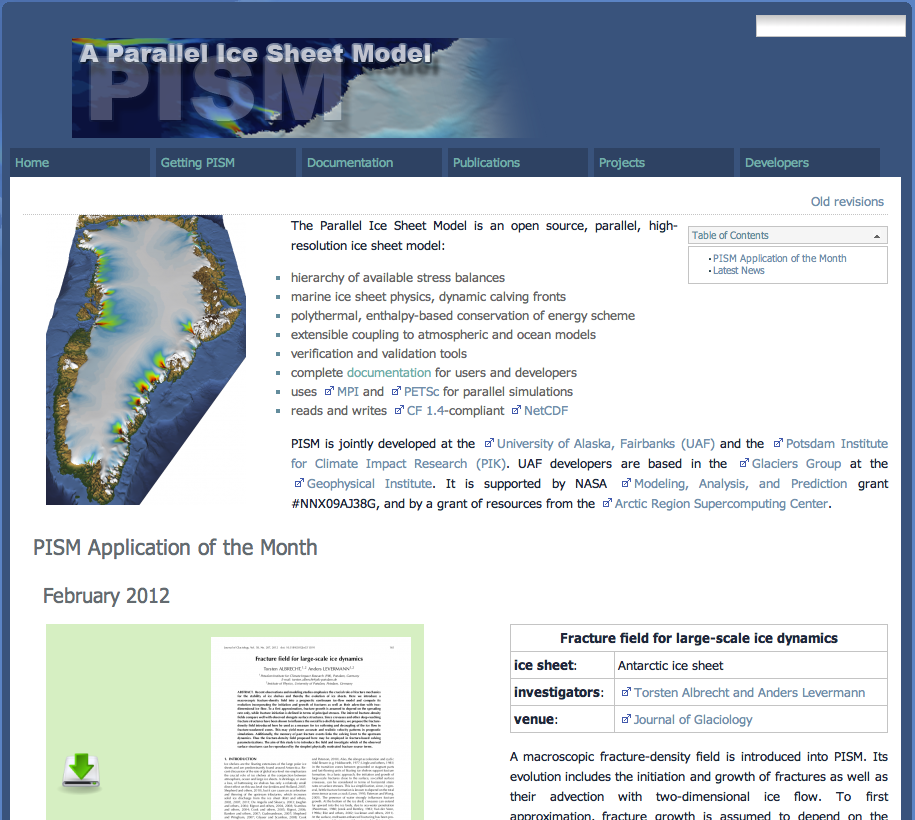
\includegraphics[width=50mm]{pismdocs.png}
    \end{column}
    \begin{column}{70mm}
      \begin{itemize}
      \item website: \alert{www.pism-docs.org}
      \item PISM runs on Linux, Unix, and Mac OSX: laptops to supercomputers
      \item stable releases once a year
      \item designed with usability in mind
      \item comprehensive User's Manual with real modeling examples
      \item \url{help@pism-docs.org}
      \end{itemize}
    \end{column}
  \end{columns}
\end{frame}


\begin{frame}
  \frametitle{PISM: power user's point of view}
  \begin{itemize}
  \item everything is parallel (PETSc and MPI)
    \begin{itemize}
    \item[$\circ$] whole Antarctica at 5 km resolution
    \item[$\circ$] whole Greenland at 1 km resolution for 100 model years
      \begin{itemize}
      \item $\approx$ 100k processor-hours on 512 cores at ARSC
      \end{itemize}
    \item[$\circ$] New Zealand LGM ice sheet at 500 m resolution (N.~Gollege at VUW)
    \end{itemize}
  \item effective, well-tested physics
    \begin{itemize}
    \item[$\circ$] shallow hybrid for stress balance
    \item[$\circ$] enthalpy method for conservation of energy
    \end{itemize}
  \item open source (GPL)
    \begin{itemize}
    \item[$\circ$] hosted at \texttt{github.com/pism/pism}
    \item[$\circ$] modular (library-like) and extensible C++ code base
    \item[$\circ$] documented source code (\texttt{doxygen})
    \end{itemize}
  \end{itemize}
\end{frame}


\begin{frame}
  \frametitle{who supports development?}
  \begin{itemize}
  \item supported by the NASA Modeling, Analysis and Prediction grant NNX09AJ38G
   (2009--2013)
  \item 2003--2008: earlier NASA grant
  \item since April 2011: jointly developed by UAF and the Potsdam
    Institute for Climate Impact Research (PIK)
  \item a \emph{community} of developers \dots likely to expand?
  \end{itemize}
\end{frame}


\begin{frame}
  \frametitle{a community of users and developers}
 \begin{center}
    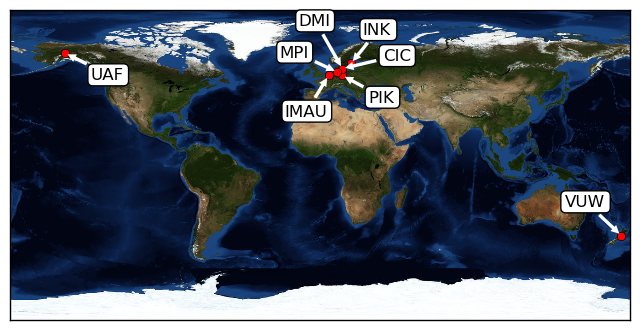
\includegraphics[width=120mm]{pism-users-map.png}
  \end{center}
\end{frame}


\begin{frame}
  \frametitle{publications}

  \begin{itemize}
  \item in the 17 months since the start of 2011: \alert{14 papers} using PISM have been published or are ``in press''
  \item see the website:
    \begin{center}
    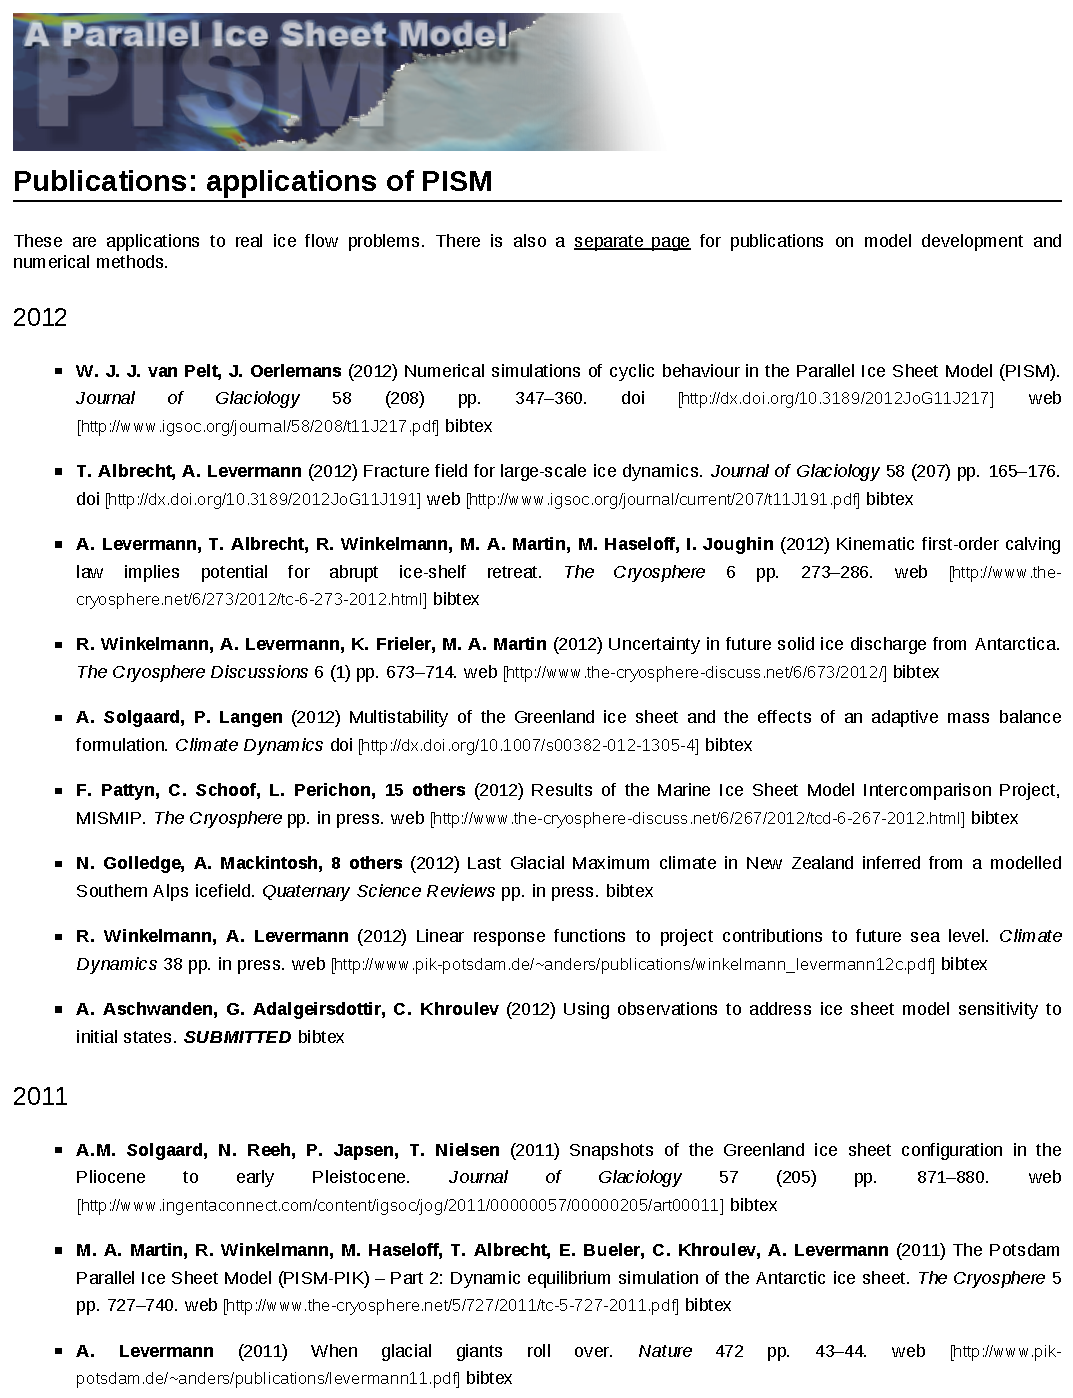
\includegraphics[height=0.65\textheight]{publications}
    \end{center}
  \end{itemize}
\end{frame}


\begin{frame}
  \frametitle{one project per month featured at website}
  \begin{center}
    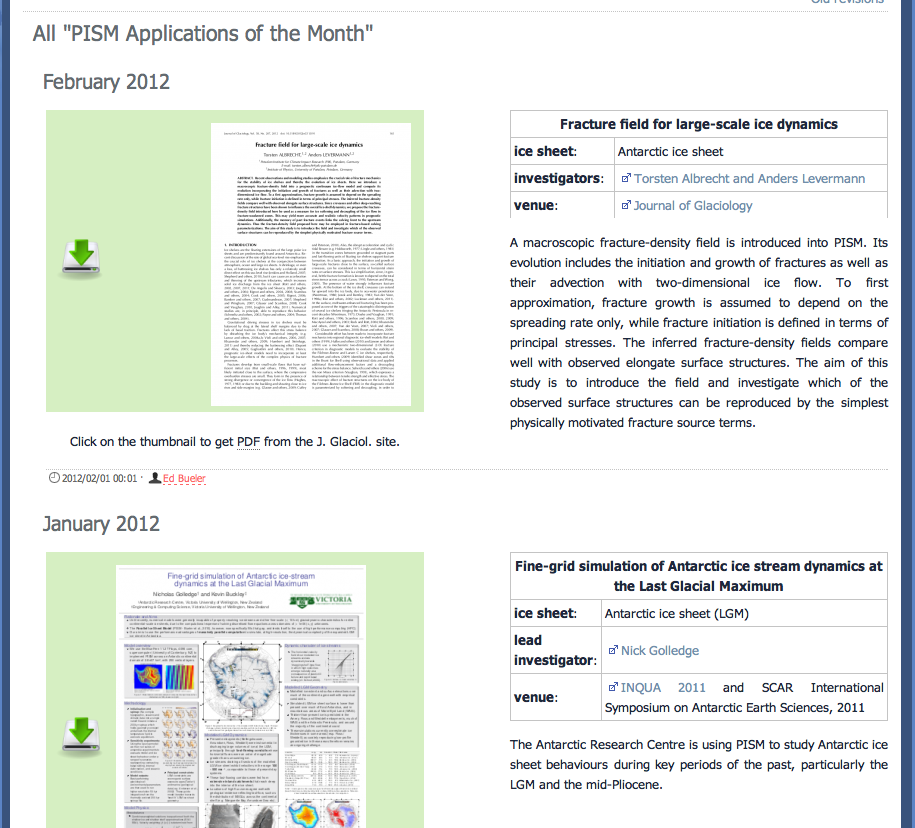
\includegraphics[height=0.75\textheight]{application-of-the-month.png}
  \end{center}
\end{frame}


\begin{frame}
  \frametitle{minimal history}
  \begin{itemize}
  \item 1984--2001: Craig Lingle does ice sheet/stream modeling in AK
  \item 2002--2004:
    \begin{itemize}
    \item[$\circ$] Craig recruits Jed Brown and me as developers
    \item[$\circ$] Jed decides on PETSc
    \end{itemize}
  \item 2005: first draft is ``COMMVNISM''
    \begin{itemize}
    \scriptsize
    \item[$\circ$] \alert{C++ Object-oriented Multi-Modal Verifiable Numerical Ice Sheet Model}
    \normalsize
    \end{itemize}
  \item 2006: first PISM release on \texttt{gna.org}
  \item 2008:
    \begin{itemize}
    \item[$\circ$] Constantine
    \item[$\circ$] PIK visits Alaska \dots branch
    \end{itemize}
  \item 2009: Andy
  \item 2011:
    \begin{itemize}
    \item[$\circ$] merge PISM-PIK
    \item[$\circ$] move to \texttt{github.com}
    \end{itemize}
  \end{itemize}
\end{frame}


\begin{frame}
  \frametitle{who answers \texttt{help@pism-docs.org}?}
  \begin{columns}
    \begin{column}{0.5\textwidth}
      \begin{center}
      %\includegraphics[width=1.0\textwidth]{}
      FIXME
      
      Constantine Khroulev
      \end{center}
    \end{column}
    \begin{column}{0.5\textwidth}
      \begin{center}
      %\includegraphics[width=1.0\textwidth]{}
      FIXME
      
      Andy Aschwanden
      \end{center}
    \end{column}
  \end{columns}

\end{frame}


\section[latest release]{latest release  (5 slides)}

\begin{frame}
  \frametitle{\texttt{0.5} release of PISM in June 2012}

  \begin{itemize}
  \item get pre-release \alert{now}:
    \begin{center}
    \texttt{git clone git://github.com/pism/pism.git pism0.5}
    \end{center}
  \item June ``official'' release after more testing, documentation
    \begin{itemize}
    \item[$\circ$] watch for CYROLIST announcement
    \item[$\circ$] (\dots do ``\texttt{git pull}'' and recompile then)
    \end{itemize}
  \item changelog from \texttt{pism0.4}:
    \begin{itemize}
    \item[$\circ$] more improvements to usability than new features
    \item[$\circ$] requires PETSc 3.2
    \item[$\circ$] \texttt{-o\_format [netcdf4\_parallel, pnetcdf]}
    \item[$\circ$] good calendar handling
    \item[$\circ$] improved documentation of climate forcing code
    \end{itemize}
  \end{itemize}
\end{frame}


\begin{frame}
  \frametitle{\texttt{0.5} update: NetCDF4 means bigger scales}

\vspace{-1mm}
  \begin{itemize}
  \item previous limitation: can't write very large ($\sim$ 4 Gb) model results
  \item \emph{new}: optional use of parallel NetCDF4 or \texttt{pnetcdf}
  \item \emph{get}: 1km Greenland runs for 100 model years
    \scriptsize
    \begin{itemize}
    \item[$\circ$] $10^9$ temperature and velocity unknowns
    \end{itemize}
    \normalsize
  \end{itemize}
  
    \vspace{-2mm}
    \begin{center}
    \includegraphics[width=1.0\textwidth]{csurf_insar_pism_all_4000px.png}
    \end{center}
\end{frame}


\begin{frame}
  \frametitle{\texttt{0.5} update: the Ross ice shelf example}

\begin{columns}
\begin{column}{0.7\textwidth}
\vspace{-5mm}
  \begin{itemize}
  \item ``diagnostic'' ice shelf example in User's Manual
  \item based on extract from 5km ALBMAP and MEASURES (2011) data
    \begin{itemize}
    \item[$\circ$] not old EISMINT-Ross data
    \end{itemize}
  \end{itemize}

\vspace{2mm}
  \animategraphics[autoplay,loop,height=5.5cm]{1}{figures/rossquiver}{0}{2}

\end{column}

\begin{column}{0.3\textwidth}
      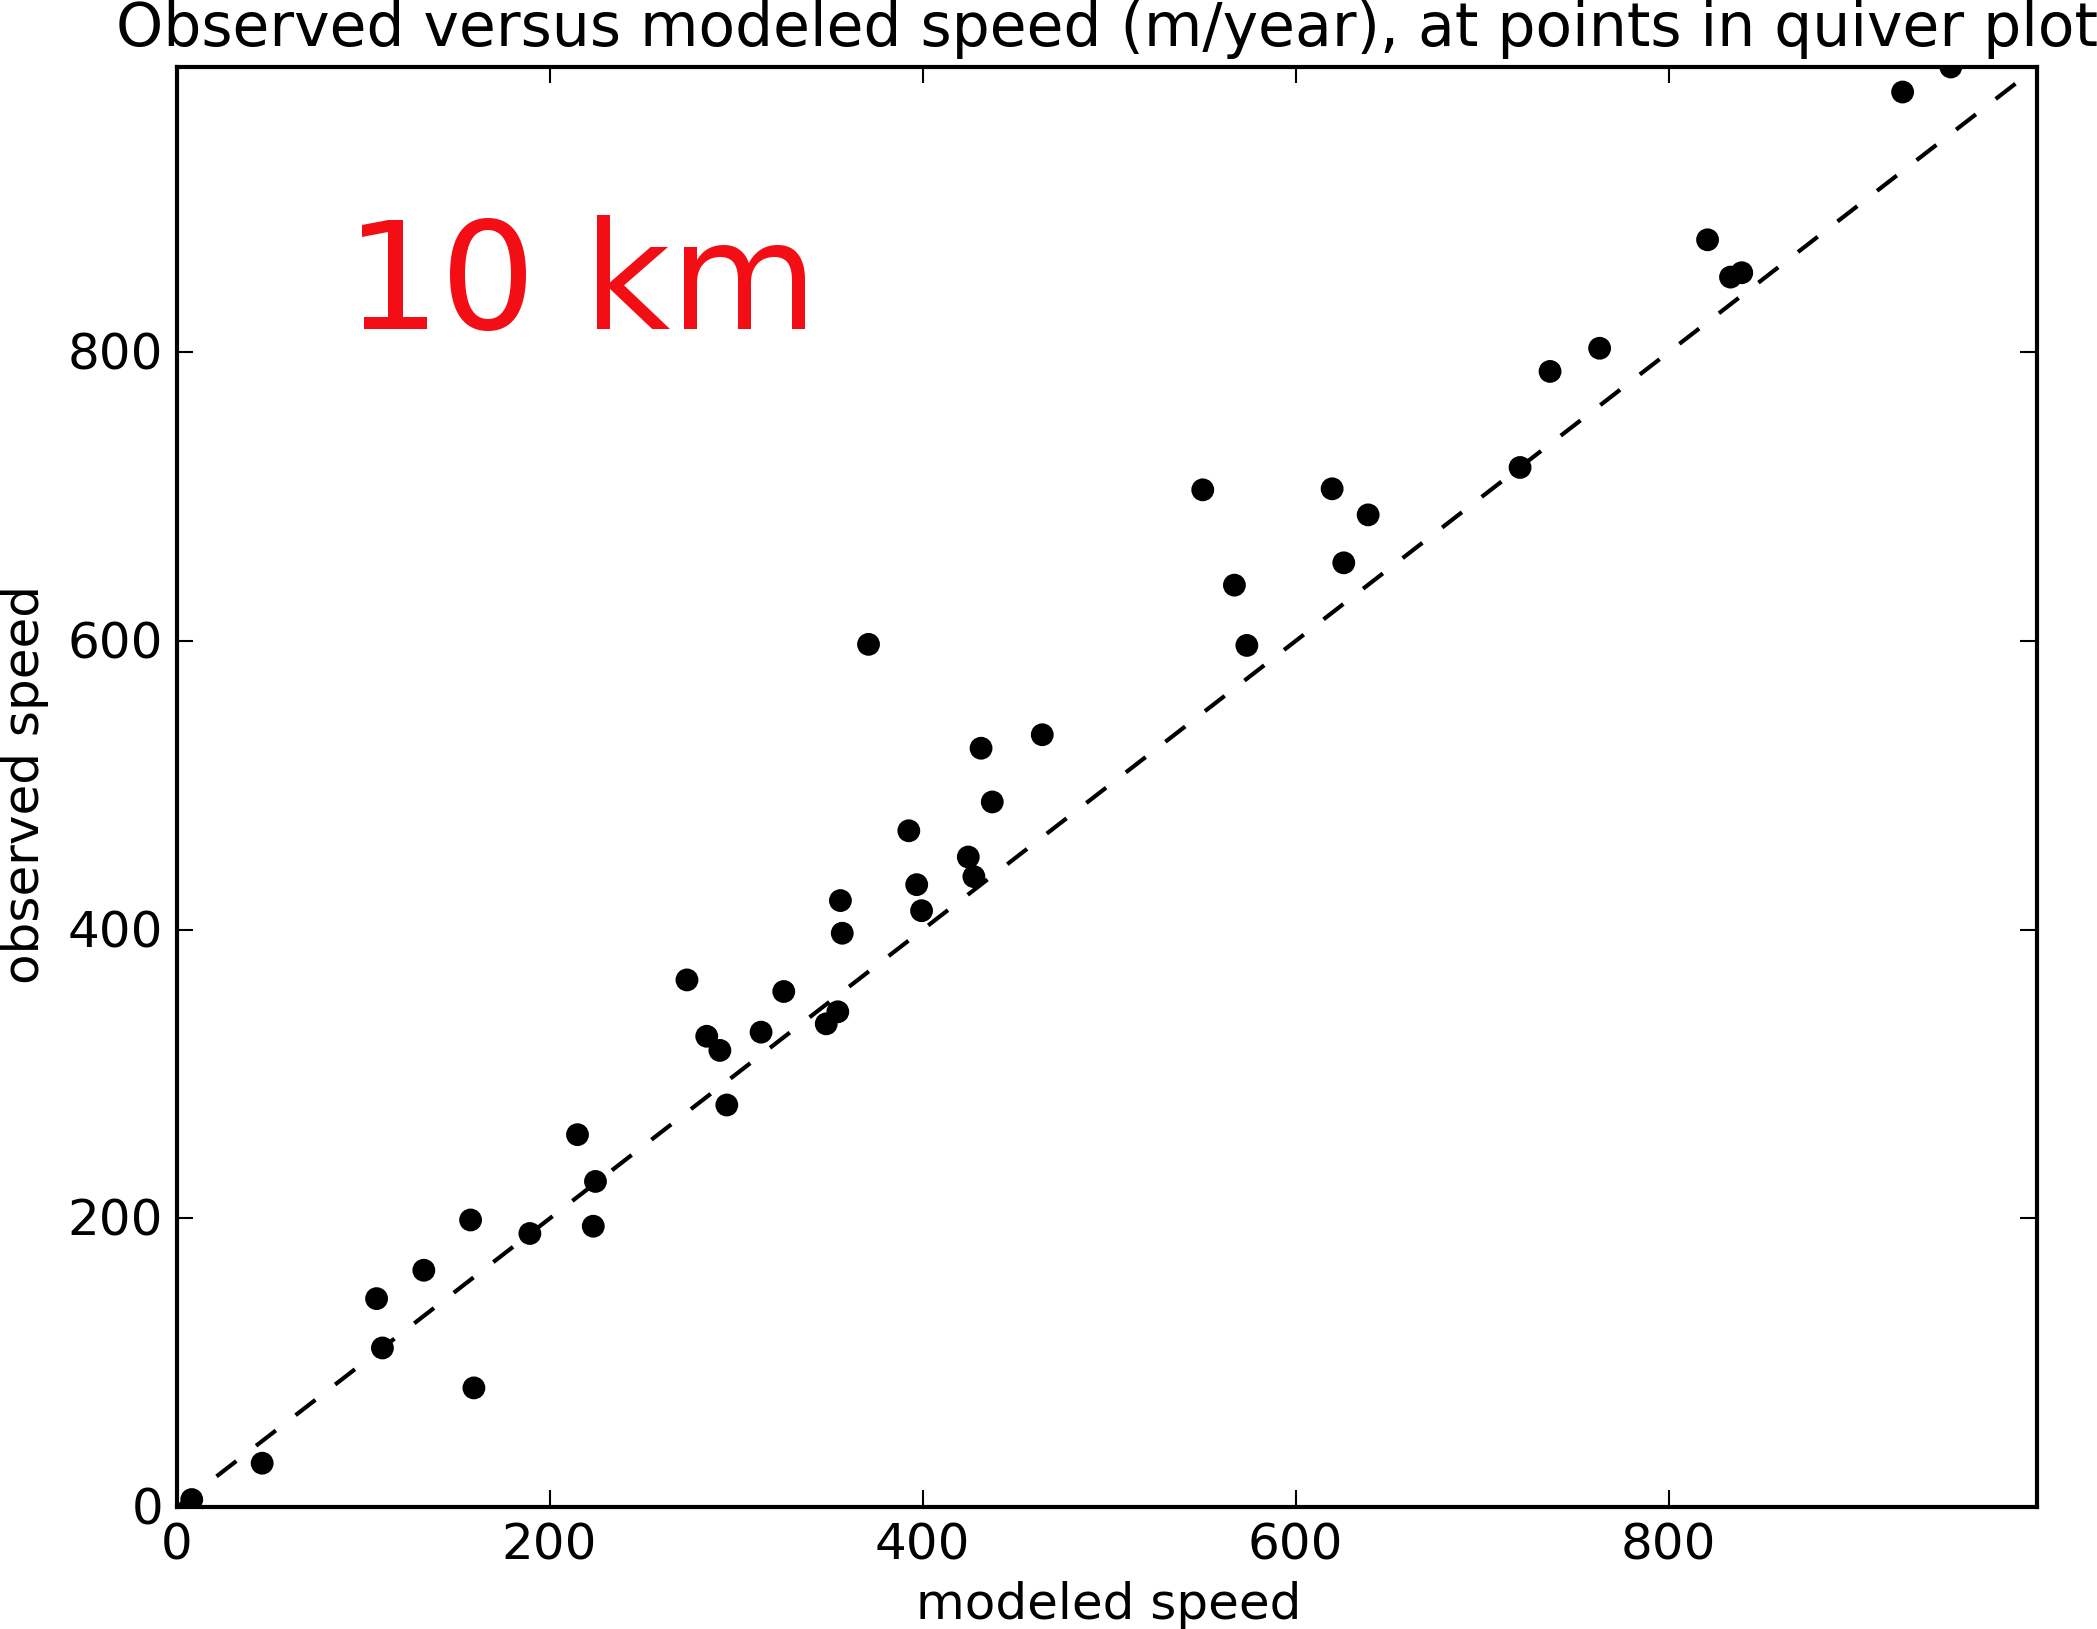
\includegraphics[width=0.8\textwidth]{rossscatter_10km.png}\\
      \rule{0pt}{5mm}\\
      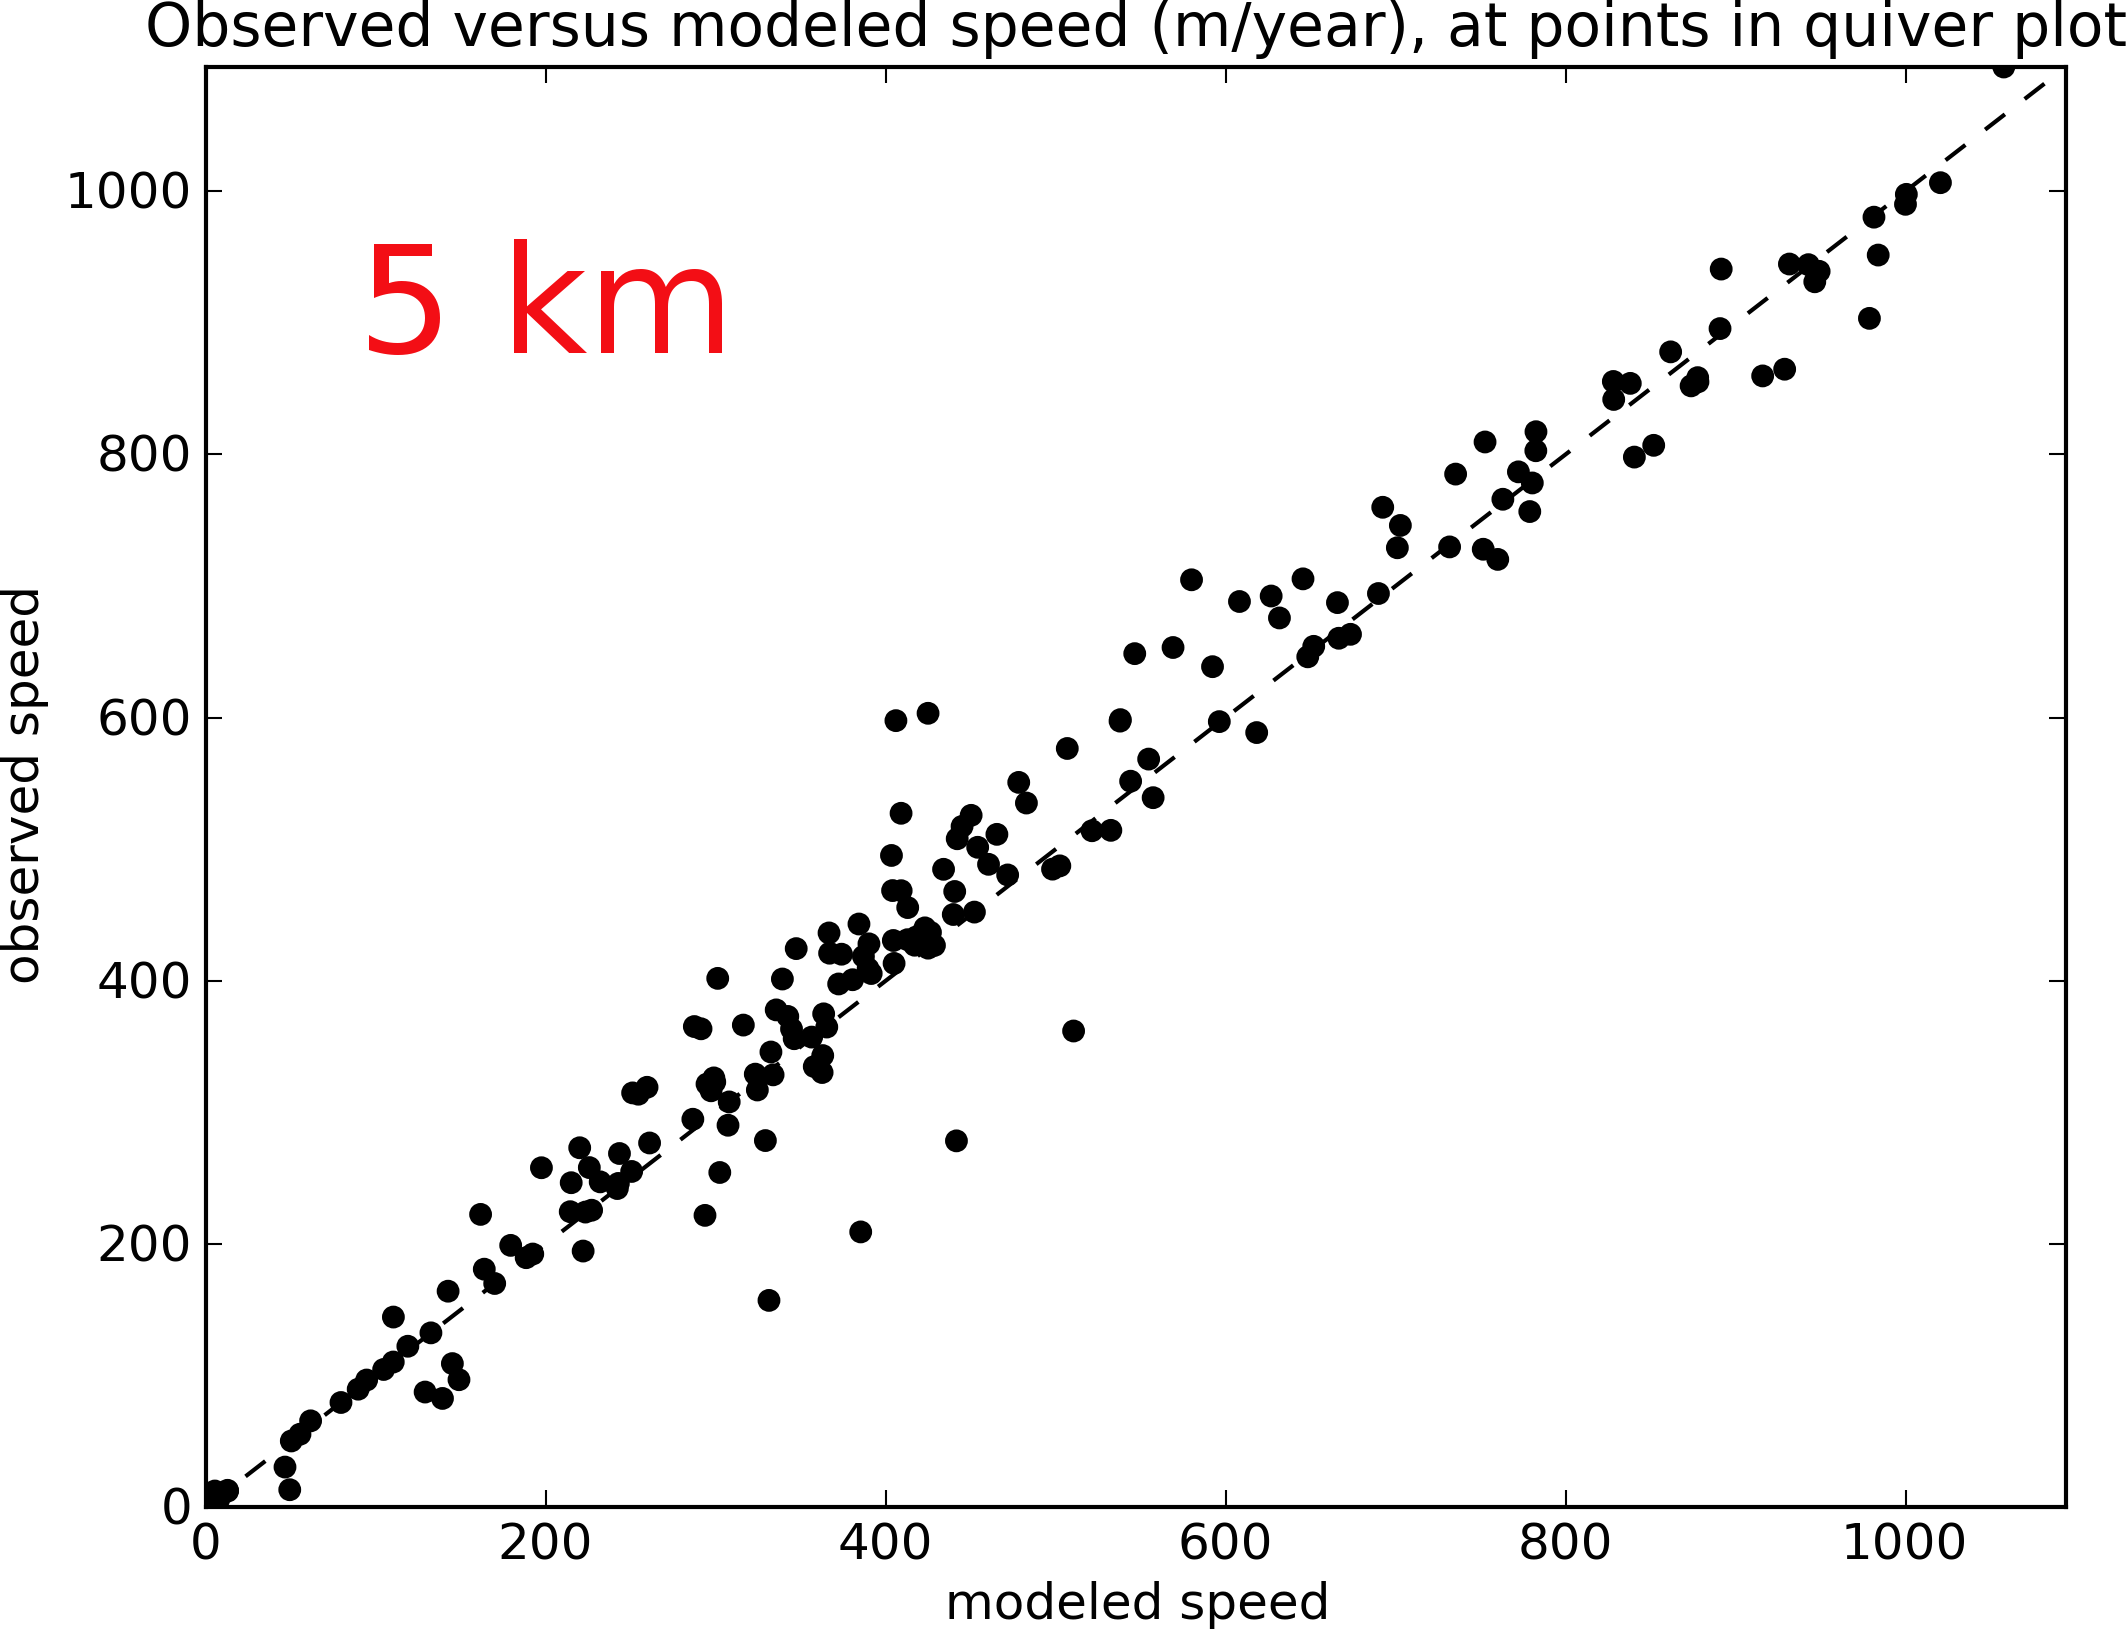
\includegraphics[width=0.8\textwidth]{rossscatter_5km.png}\\
      \rule{0pt}{5mm}\\
      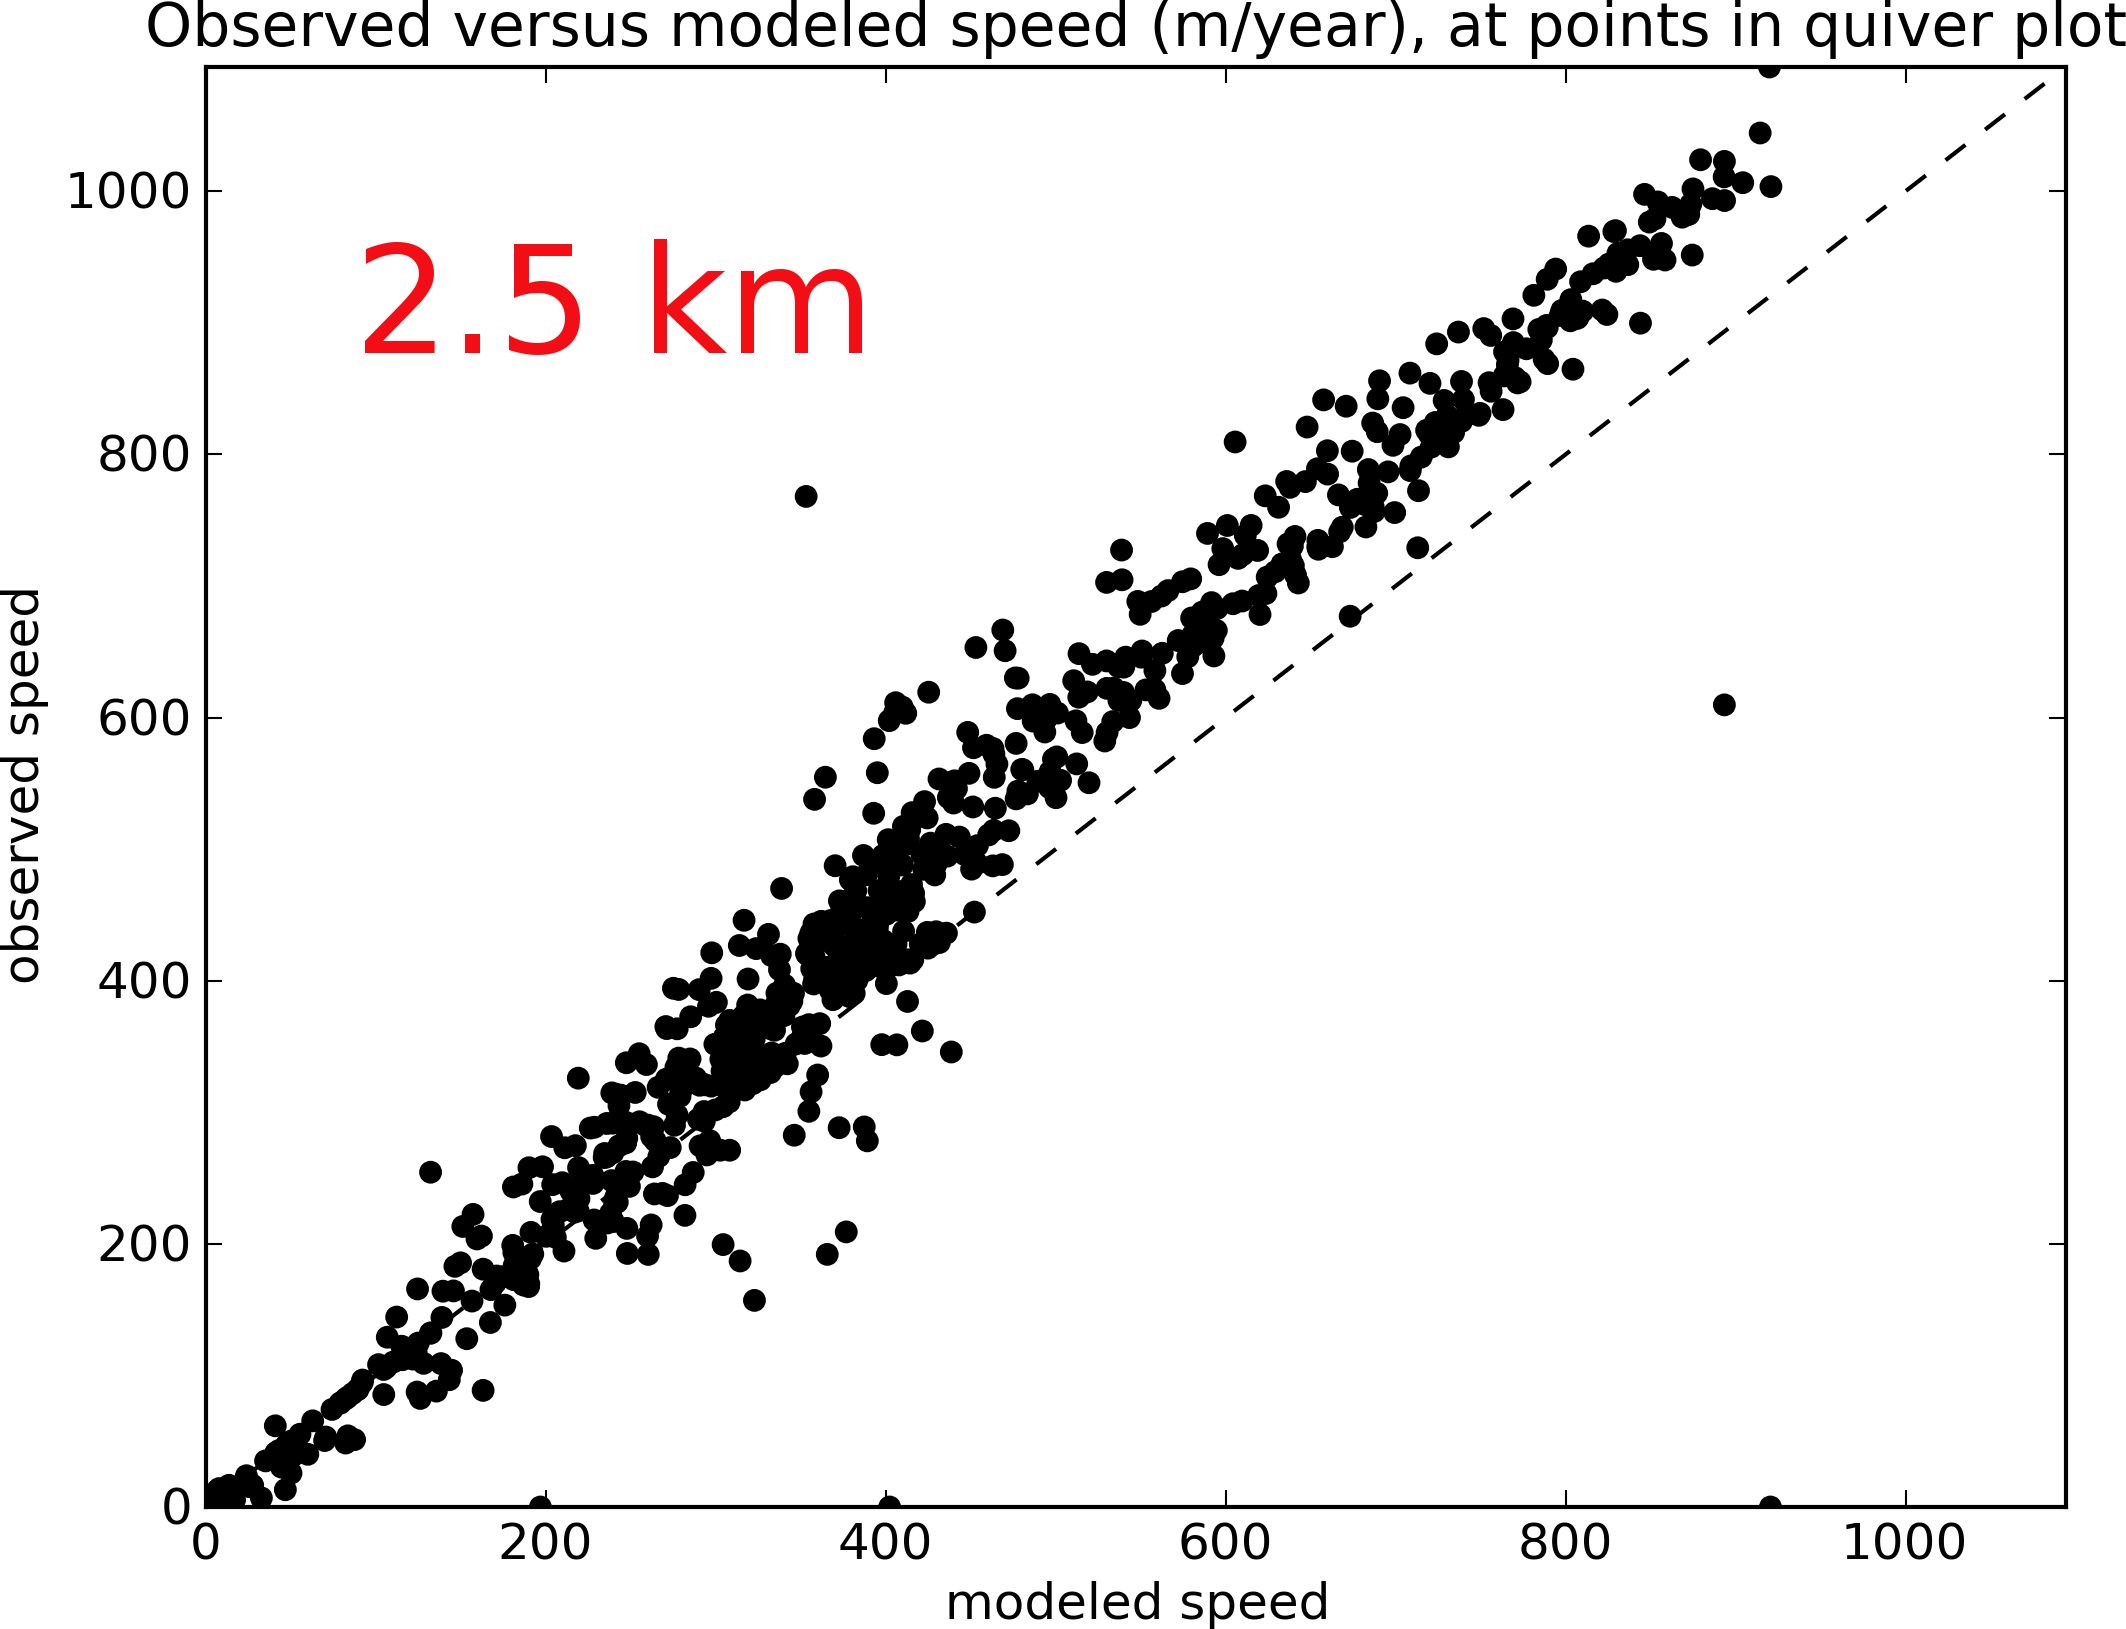
\includegraphics[width=0.8\textwidth]{rossscatter_2_5km.png}
\end{column}
\end{columns}
\end{frame}


\begin{frame}
  \frametitle{\texttt{0.5} update: regional tools}
  \framesubtitle{(e.g.~Jakobshavn outlet glacier)}
  
\begin{columns}
\begin{column}{0.5\textwidth}
\begin{itemize}
\vspace{-2mm}
\small
\item regional models allow large parameter studies on fine grids
\item automated drainage basin identification from DEM (below)
\end{itemize}

\vspace{2mm}

  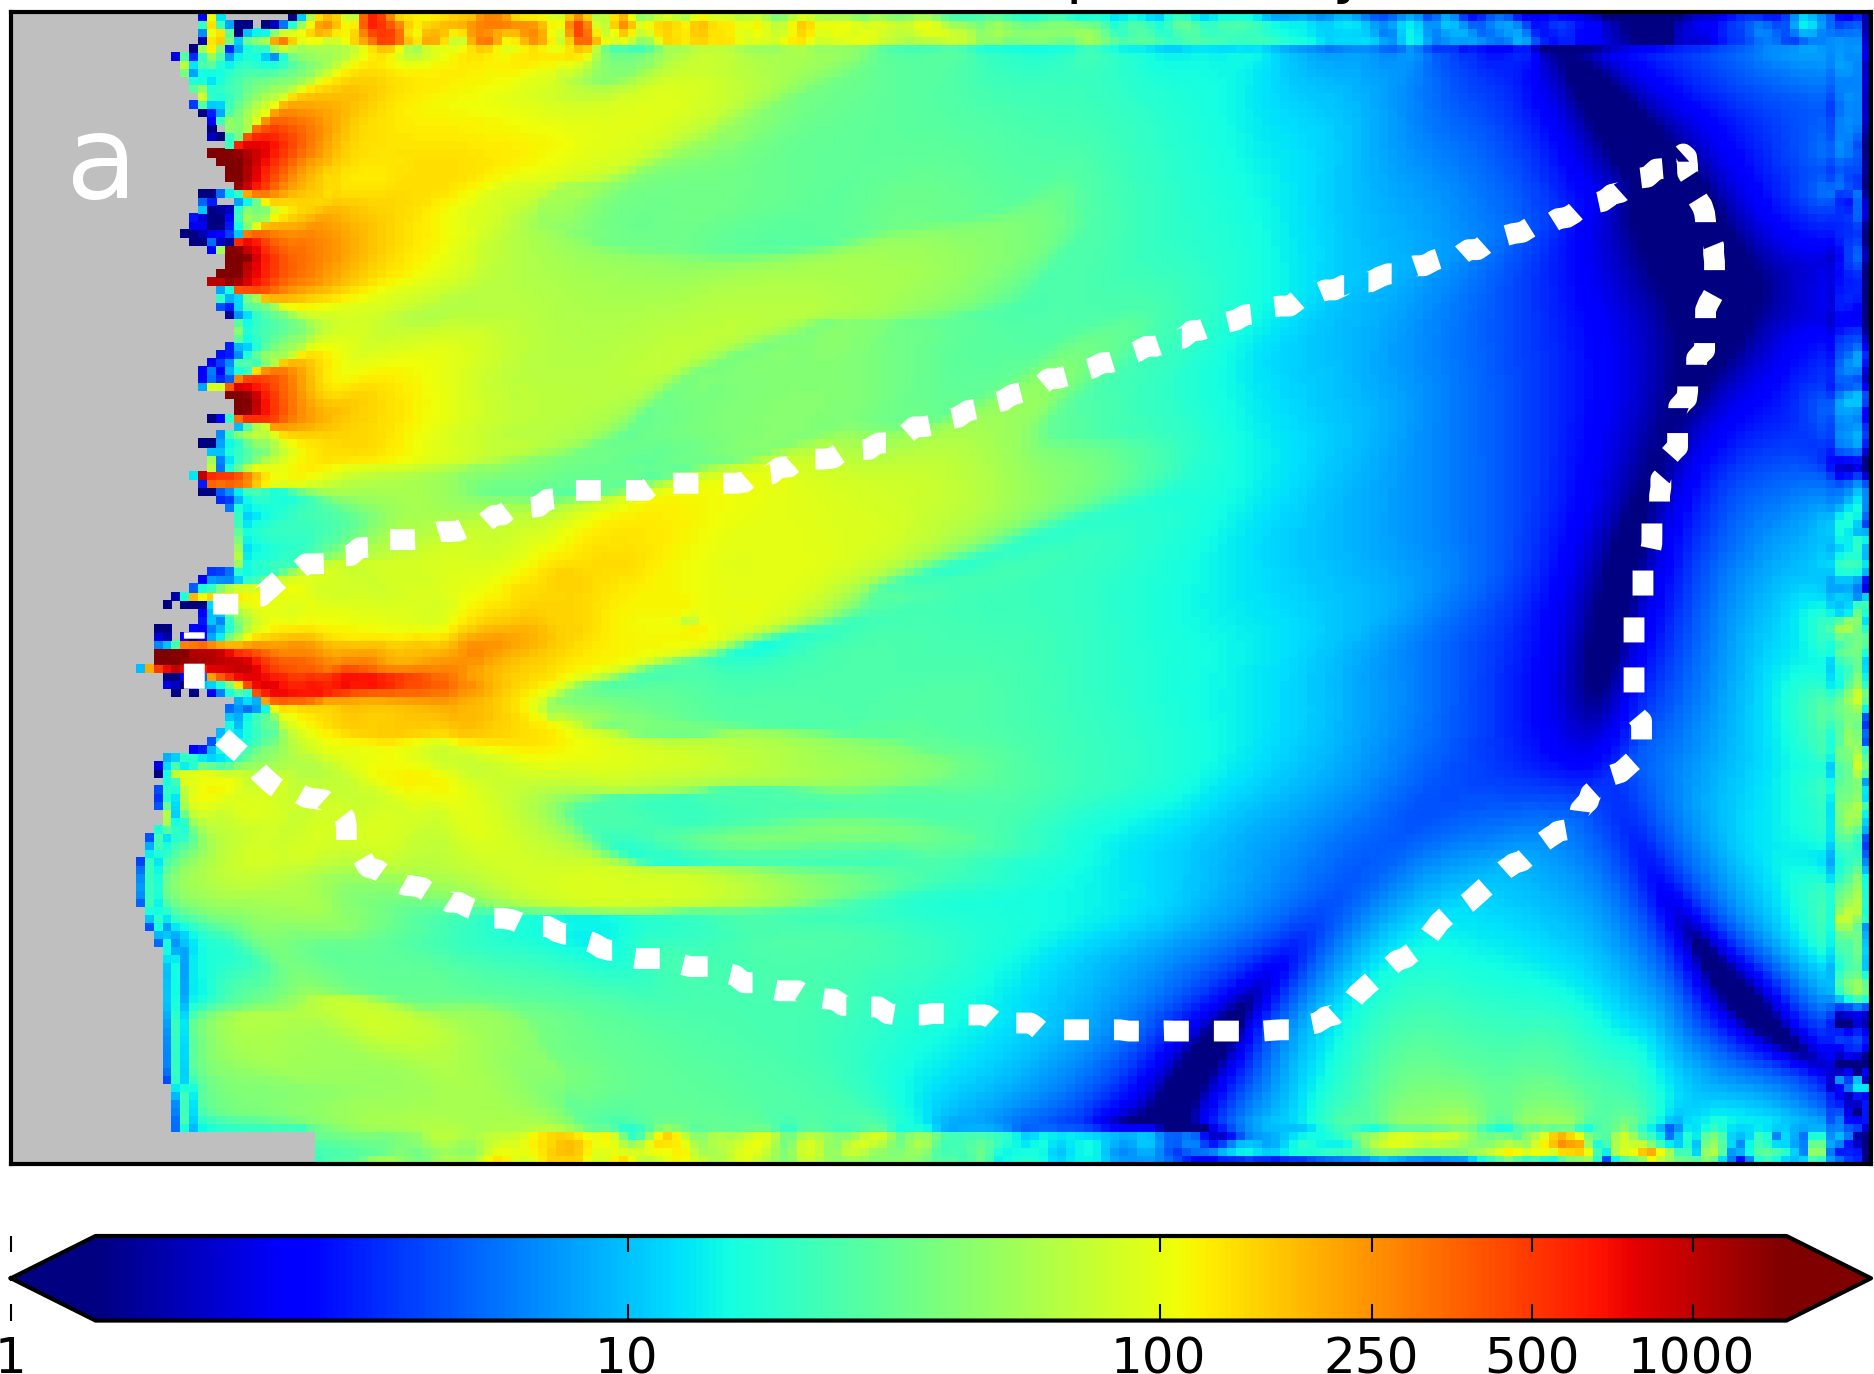
\includegraphics[width=0.85\textwidth]{jako_3km}

\end{column}

\begin{column}{0.5\textwidth}
FIXME: figure in Andy email
\end{column}
\end{columns}

\begin{center}
\scriptsize \texttt{git clone git://github.com/pism/regional-tools.git}
\end{center}
\end{frame}



\begin{frame}
  \frametitle{update \texttt{0.5}: some option combinations}
  \begin{itemize}
  \item running PISM and setting the grid (alternatives):
    %\vspace{-2mm}
    \small

    \texttt{\$ pismr -boot\_file data.nc -Mx 76 -My 141 -Mz 101 -Mbz 11 $\backslash$}
    
    \texttt{\phantom{foobar} -Lz 4000 -Lbz 2000}

    \texttt{\$ pismr -i prev-state.nc}
    \normalsize
  \item setting the duration (alternatives):
    %\vspace{-2mm}
    \small

    \texttt{\dots\quad -ys YEAR -ye YEAR}
    
    \texttt{\dots\quad -ys YEAR -y DURATION}
    \normalsize
  \item a sliding model possibility:
    %\vspace{-2mm}
    \small

    \texttt{\dots\quad -ssa\_sliding -topg\_to\_phi 5.0,30.0,-300.0,700.0 $\backslash$}
    
    \texttt{\phantom{foobar} -pseudo\_plastic -pseudo\_plastic\_q 0.25 $\backslash$}
    
    \texttt{\phantom{foobar} -plastic\_pwfrac 0.98 }
    \normalsize

  \item ice shelf calving front model (alternatives):
    %\vspace{-2mm}
    \small

    \texttt{\dots\quad -ocean\_kill bar.nc -cfbc -kill\_icebergs}

    \texttt{\dots\quad -eigen\_calving -eigen\_calving\_K 1e17 $\backslash$}
    
    \texttt{\phantom{foobar} -thickness\_calving -calving\_at\_thickness 50.0}
    \normalsize
  \end{itemize}
\end{frame}


\section[UAF work]{some recent UAF work (3 slides)}


\begin{frame}
  \frametitle{enthalpy model}
  \framesubtitle{main point: basal melt rate from better energy conservation}

  \begin{center}
    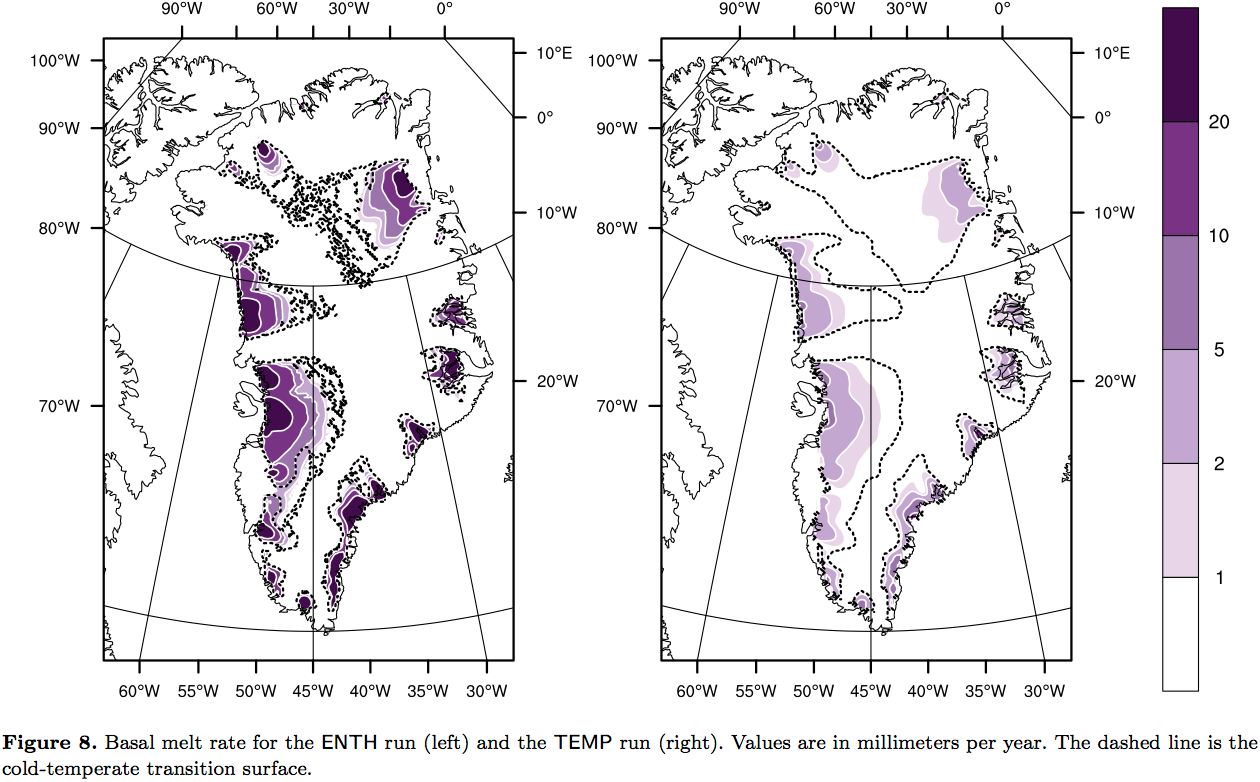
\includegraphics[height=0.7\textheight]{enthalpy-model.png}
  \end{center}

\begin{flushleft}
\scriptsize \textbf{Aschwanden, Bueler, Khroulev, Blatter} (2012) \emph{An enthalpy
      formulation for glaciers and ice sheets}, J. Glaciol. 58 (209), 441--457.
\end{flushleft}
\end{frame}


\begin{frame}
  \frametitle{analysis of ``initial states'' for Greenland}
  \framesubtitle{main point: good agreement with observed-period observations without inversion}

  \begin{columns}
  \begin{column}{0.4\textwidth}
  \begin{itemize}
  \item using HIRHAM 1989--2009 mean air temp.~and SMB 
  \item using ice2sea 1km bed topography
  \end{itemize}

    \includegraphics[width=0.85\textwidth]{csurf_insar_pism_all_4000px}
  \end{column}
  \begin{column}{0.6\textwidth}
    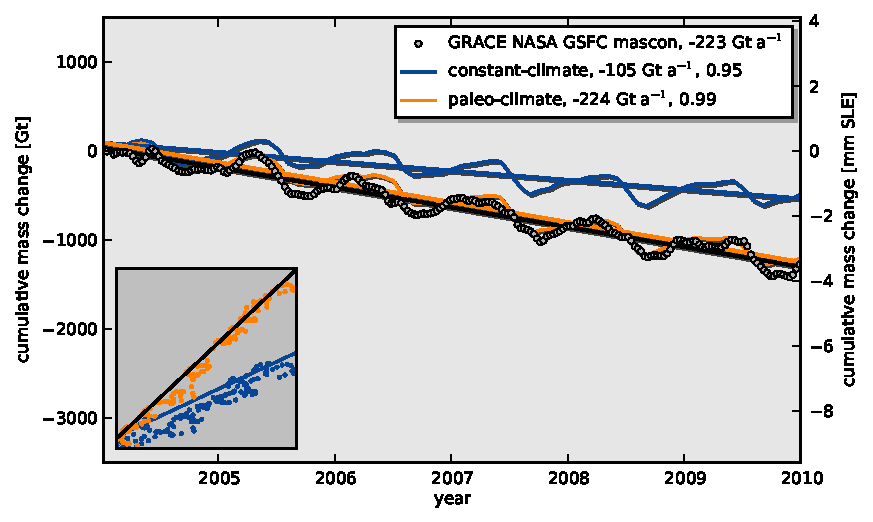
\includegraphics[width=1.0\textwidth]{ts_mass_2004-2009}
  \end{column}
  \end{columns}

  \begin{flushleft}
  \scriptsize \textbf{Aschwanden, A{\dh}algeirsd{\'o}ttir, Khroulev} (submitted) \emph{Using observations to address ice sheet model sensitivity to initial states}
 \end{flushleft}
\end{frame}


\begin{frame}
  \frametitle{inversion of SSA (and hybrid) for basal shear stress}
  \framesubtitle{main point: inversion must be done with care}

  \begin{itemize}
  \item inverse modeling (lead by David Maxwell and Marijke Habermann)
  \item uses new tools (written in Python)
  \item shares code with PISM
  \item well under way
  \end{itemize}

  \begin{center}
    FIXME: FIGURE
    %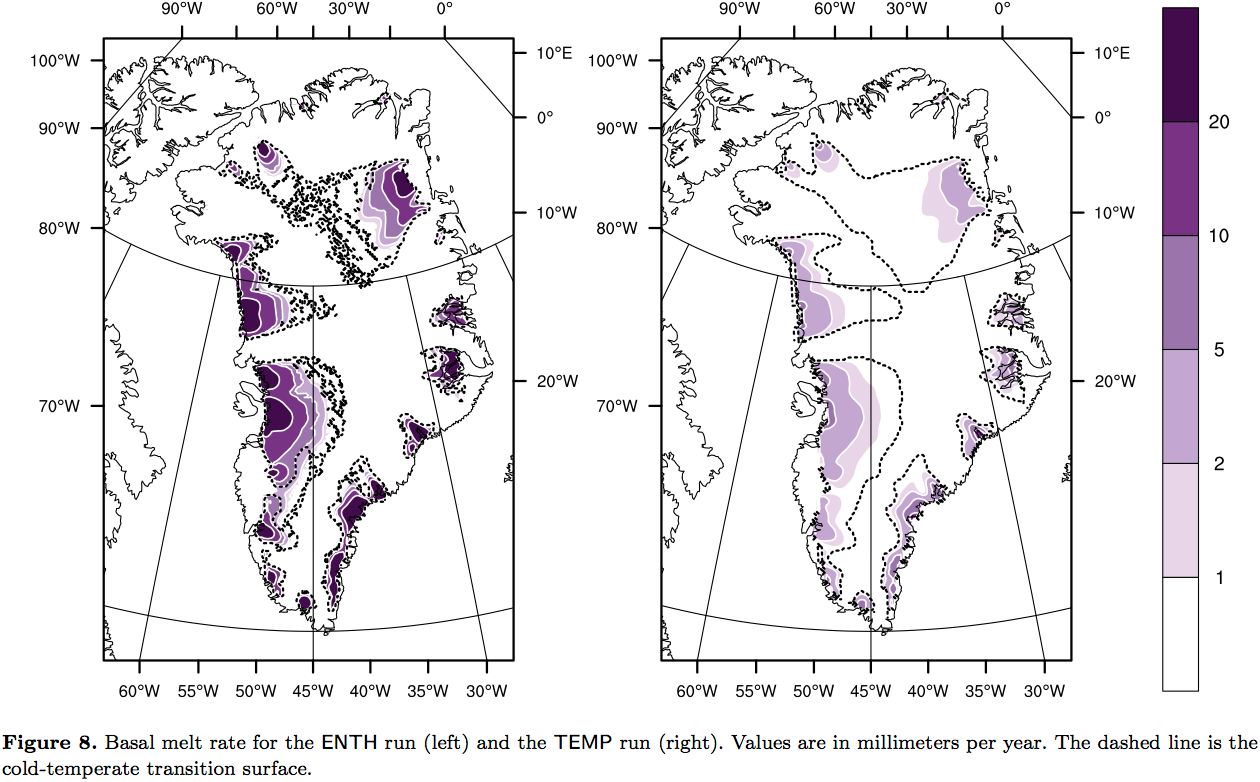
\includegraphics[height=0.7\textheight]{enthalpy-model.png}
  \end{center}

\begin{flushleft}
\scriptsize \textbf{Habermann, Maxwell, Truffer} (2012) \emph{Reconstruction of basal properties in ice sheets using iterative inverse methods}, J. Glaciol., to appear
\end{flushleft}
\end{frame}


\section[to improve]{what we know we need to improve (4 slides)}

\begin{frame}
  \frametitle{to improve: better grounding line motion}
  \begin{itemize}
  \item foo
  \end{itemize}
\end{frame}

\begin{frame}
  \frametitle{to improve: add ``higher-order'' stress balance}
  \begin{itemize}
  \item ``higher-order stress balance'' means one that balances more stresses, in one solution process, than in either the SIA or SSA stress balances
    \begin{itemize}
    \item[$\circ$]  \emph{note}: Stokes stress balance is \emph{not} planned for PISM
    \end{itemize}
  \item a Blatter stress balance solver$^{*}$ is present in the PISM dev branch
    \begin{itemize}
    \item[$\circ$] but all it can do is ISMIP-HOM
    \item[$\circ$]
    \end{itemize}    
  \item it is unclear how ``higher-order'' is the current SIA+SSA hybrid
  \end{itemize}

 \begin{flushleft}
   \scriptsize
    $^{*}$see Jed's paper \textbf{Brown et al},
    \emph{Achieving textbook multigrid efficiency for hydrostatic ice sheet
      flow}, submitted to SIAM J. Scientific Computing.
  \end{flushleft}
\end{frame}


\begin{frame}
  \frametitle{to improve: better hydrology model}
  \begin{itemize}
  \item foo
  \end{itemize}
\end{frame}


\begin{frame}
  \frametitle{to improve: better transport schemes}
  \begin{itemize}
  \item foo
  \end{itemize}
\end{frame}


\section[where to?]{where is PISM going?}

\begin{frame}
  \frametitle{where is PISM going?}
  \framesubtitle{(where will you lead it?)}

\begin{itemize}
  \item everyone can (and should) branch the code and try new things
  \item merging successful ideas from branches
    \begin{itemize}
    \item[$\circ$] is really important!
    \item[$\circ$] requires decisions and synoptic view of code
    \item[$\circ$] central scientific programmer (= Constantine Khroulev) is vital
    \end{itemize}
  \item \alert{thanks for listening!}

\bigskip\bigskip

  \item where are we going?  let's talk right now
\end{itemize}

\end{frame}



\end{document}
